% Why prediction is important?
\label{sec:prediction}
This section further motivates predictive false sharing and explains how to support it in the runtime system.  

\subsection{Overview}
%\begin{figure*}[!htb]
\label{sec:predictoverview}

\begin{figure}[!t]
\begin{center}
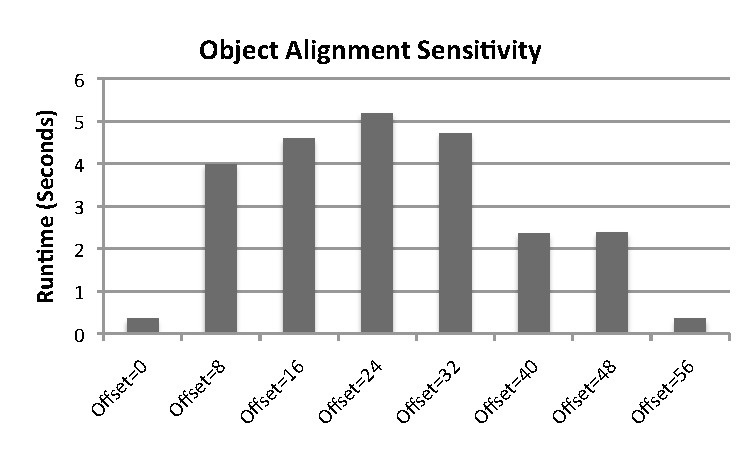
\includegraphics[width=5in]{predator/figure/perfsensitive}
\end{center}
\caption{
Performance of the linear\_regression benchmark (from Phoenix)  is highly sensitive to the memory layout between the (potentially) falsely-shared object and corresponding cache lines. 
\label{fig:perfsensitive}}
\end{figure}

The appearance of false sharing depends on 
the memory layout between objects and corresponding cache lines. The performance of a real example, linear\_regression, is shown in Figure~\ref{fig:perfsensitive}: 
When the offset of the starting address between the potentially falsely-shared object and corresponding cache lines is $0$ or $56$ bytes, there is no false sharing; 
When the offset is $24$ bytes, we see the most severe performance effect caused by false sharing. 
The performance difference caused by false sharing can affect the performance as large as $15\times$ on an 8-core machine. 

Existing detection tools can only report observed false sharing. That means, they may miss such a very severe false sharing problem that could occur in the wild if the offset of the starting address was $0$ bytes or $56$ bytes in their test environment. \Predator{} overcomes this shortcoming by accurately predicting potential false sharing, without the need of occurrences. 

\begin{figure*}
\begin{center} 
\subfigure[No false sharing]{%
   \label{fig:nofs}
   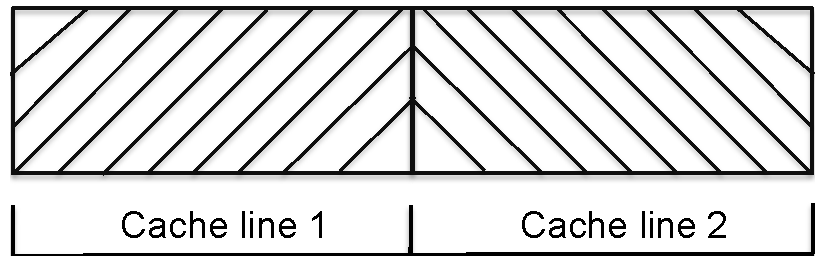
\includegraphics[width=0.24\textwidth]{predator/figure/Potential1}
}%
\hspace{10pt}
\subfigure[False sharing with larger cache size]{%
   \label{fig:fslarger}
   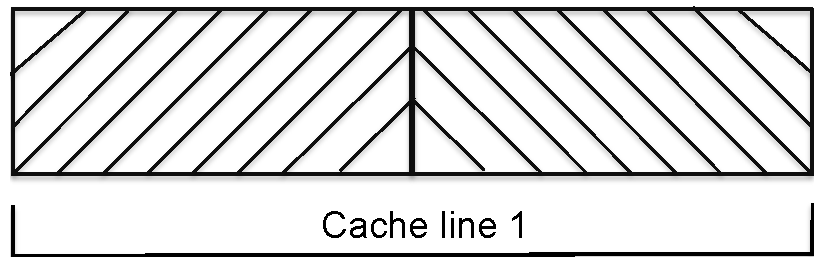
\includegraphics[width=0.24\textwidth]{predator/figure/Potential2}
}%
\hspace{10pt}
\subfigure[False sharing with different memory layout]{%
   \label{fig:fsnoalignment}
   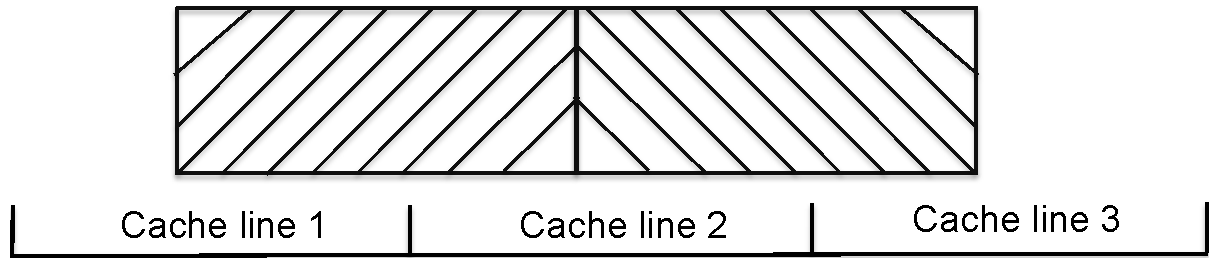
\includegraphics[width=0.36\textwidth]{predator/figure/Potential3}
}%
\end{center}
%\includegraphics{fig/potential.pdf}
\caption{False sharing under different environments.}
\label{fig:potentialfalsesharing}
\end{figure*}

\Predator{} predicts {\it potential false sharing}, which does not manifest in the current execution but may appear and greatly affect performance of programs in a slightly different environment.

Figure~\ref{fig:potentialfalsesharing} shows a simplified example why occurrences of false sharing can change in different situations. 
In this figure, two rectangles with different patterns
represents two portions of the same object, updated by different threads. In Figure~\ref{fig:nofs}, there is no false sharing when thread T1 only updates 
``cache line 1'' and T2 only updates ``cache line 2''.
However, false sharing appears in one of the following cases, even with the same
access pattern. 

\begin{itemize}
\item
Doubling cache line size (Figure~\ref{fig:fslarger}). When the size of a cache line doubles, both T1 and T2 access the same cache line concurrently, thus causing false sharing.

\item
Different starting address of an object(Figure~\ref{fig:fsnoalignment}).  
When the starting address of this object is not aligned with the starting address of the first cache line, then T1 and T2 can update the second cache line simultaneously, causing a false sharing problem. 
%When some dynamic property changes the starting address of this object so that it 
%is not aligned with the starting address of the first cache line, 
\end{itemize} 

\Predator{} predicts whether programs can have potential false sharing in one of these two situations, where they can be caused by different dynamic properties. These dynamic properties include choosing a different compiler, enabling different compiler optimizations, using a different memory allocator, adding or removing code involving in memory allocations, switching to a different target platform with a different address mode (32-bit or 64-bit), and changing the size of cache line (64 Bytes or 128 Bytes). 
All dynamic properties, except changing the size of cache line, can lead to a different memory layout, thus can possibly affect occurrences of a false sharing problem. Thus, predicting false sharing in changing the memory layout or changing the size of cache line actually explores many possibilities caused by all of these dynamic properties.

\subsection{Basic Prediction Workflow}
\label{sec:predictionmechanism} 

%Similar to the detection part, 
\Predator{} focuses on potential false sharing that can 
cause performance problems.
It is based on two key observations. First, only accesses to 
adjacent cache lines can lead to potential false sharing, 
i.e., introducing cache invalidations when the cache line size
or an object's starting address changes.
Second, only those cache lines with a large number of cache invalidations can degrade performance.

Based on these two observations, \Predator{} develops 
the following workflow to predict potential false sharing.
Those detection optimizations listed in Section~\ref{optimization} can also be applied
to here. We do not repeat these optimizations in this section.

\begin{enumerate}
\item
Track the number of writes on different cache lines. 

\item
When the number of writes to a cache line $L$ reaches {\it Tracking-Threshold},
\predator{} tracks the detailed read and write accesses for every word on both cache line $L$ 
and its adjacent cache lines. 

\item
When the number of writes to a cache line $L$ reaches a second threshold (called as
{\it Predicting-Threshold}), 
\predator{} identifies whether there exists false sharing in $L$ and its adjacent cache lines by analyzing word accesses information collected in Step 2, which are described in 
Section~\ref{sec:evaluatingfs} in detail.

\item
If a potential false sharing is found, \predator{} starts to track cache line invalidations in order to confirm its seriousness, which are discussed in Section~\ref{sec:tracking}.
Otherwise, go back to Step 2 to track more detailed accesses.
 
\end{enumerate}

\subsection{Searching for Potential False Sharing}
\label{sec:evaluatingfs}
To describe potential false sharing in two different cases, we first introduce a concept -- ``virtual cache line''.  A virtual cache line is a contiguous memory range that spans one or more physical cache lines.  

In the case of double cache line size, a virtual line is composed of two originally contiguous cache lines, where it starts with a even number cache line.  Thus, only cache lines $2*i$ and $2*i+1$ can form a virtual cache line.  

To evaluate a potential false sharing problem that can be caused by changing memory layout, a virtual line should have the same size as an actual cache line, but with a different starting address: unlike actual cache lines, the
starting address of a virtual cache line does not need to be multiple of the cache line size. For instance, a 64-byte-long virtual line can consist of the range $[0,64)$ bytes or $[8,72)$ bytes.

To search for a potential false sharing problem, 
\Predator{} searches for a pair of hot accesses, one on $L$ and one on its previous or next cache line, based on detailed word information collected in Step 2. Two accesses happening in the same actual cache line should be detected by the normal detection mechanism, thus they can lead to actual false sharing problems but not a potential false sharing problem. 

A hot access refers to an access that has the number of read or write accesses larger than the average number of accesses. In fact, for every hot access $X$ in a specific cache line $L$, \Predator{} searches another
hot access $Y$ in $L$'s previous cache line or next cache line, satisfying the following conditions: 

\begin{itemize}
\item
$X$ and $Y$ reside on the same virtual line. 

\item
One of $X$ and $Y$ is a write access.

\item 
$X$ and $Y$ are issued by different threads.

\end{itemize}

% why it finds a pair of $X$ and $Y$ == a potential false sharing 
Whenever it finds such a pair, $X$ and $Y$, 
\Predator{} identifies a potential false sharing problem: they can degrade performance when the number of cache invalidations possibly caused by $X$ and $Y$ (on a possible virtual line), is larger than a pre-defined threshold. This approach is based on a similar observation as in detection: \emph{if a thread writes a virtual line after other threads have accessed the same virtual line, this write operation causes at least one cache invalidation}. 

However, before tracking detailed memory accesses on a specific virtual line, it is impossible to know exactly how many cache invalidations actually happen on this virtual line. Thus, \Predator{} conservatively assumes that accesses from different threads occurs in a interleaved way, with the maximum number of cache invalidations. Then \Predator{} starts to track possible cache invalidations on a virtual covering both $X$ and $Y$, described in Section~\ref{sec:tracking}.  

%According to above observation and assumption, 
%a pair of hot accesses, $X$ and $Y$, if accesses are issued in an interleaving 
%way, can generate the number of cache invalidations equaling to 
%the smaller number of accesses of $X$ and $Y$.
%Thus a false sharing problem is to be identified by \Predator{}.
  

\subsection{Verifying Potential False Sharing}
\label{sec:tracking}

\Predator{} verifies potential false sharing by tracking possible cache invalidations on a specific virtual line covering such a hot access pair, $X$ and $Y$.
%covering a pair of hot accesses found
%in Step 3.

For potential false sharing caused by double cache line size, as described in Section~\ref{sec:evaluatingfs}, a virtual line is always composed of cache line with index $2*i$ and $2*i+1$. 
\Predator{} tracks cache invalidations on a virtual line that covering $X$ and $Y$. This virtual line is unique for a given $X$ and $Y$ pair. 

However, for the case of changing memory layout, two hot accesses with distance less than the cache line size 
can actually form multiple virtual lines. 
There is thus an additional step to determine which virtual line to be tracked. 
Although a virtual line to be chosen here is never a real cache line of actual hardware because of unaligned addresses,
we utilize this virtual line to simulate the effect of changing memory layout correspondingly.


\begin{figure}
\begin{center} 
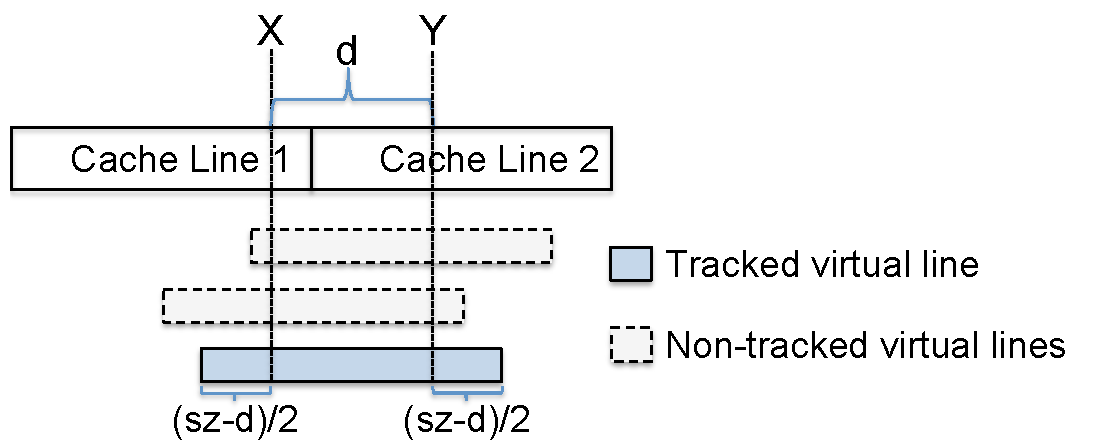
\includegraphics[width=5in]{predator/figure/trackpotential}
\end{center}
\caption{Determining a virtual line with size $sz$ according to hot accesses.}
\label{fig:trackpotential}
\end{figure}

Figure~\ref{fig:trackpotential} shows that multiple virtual lines can cover $X$ and $Y$. However, \Predator{} only chooses one of these virtual lines. \Predator{} chooses the virtual line that leaves the same space before $X$ and after $Y$. That is, the virtual line starting at location $X-((sz-d)/2)$ and ending at $Y+((sz-d)/2)$ is tracked by \Predator{}. This choice allows tracking of more possible cache invalidations caused by adjacent accesses of $X$ and $Y$. Since adjusting the starting address of a virtual line has the same effect of adjusting the starting address of an object in detecting false sharing, all cache lines related to the same object must be adjusted at the same time. \Predator{} then tracks cache invalidations based on these adjusted virtual lines.

In the end, \Predator{} can report accurately whether the change of memory layout can affect the performance or not, based on the possible number of cache invalidations. 

Currently, \predator{} only determines a specific virtual line to be tracked. However, we plan to extend this in the future work by using a much more flexible mechanism: we can choose a different virtual line after a number of accesses if the current choose cannot reveal a big number of cache invalidations.

